\documentclass{article}
\usepackage{tikz}
\begin{document}
\begin{center}
\begin{tikzpicture}
\node{Sentence}[sibling distance = 3cm, level distance = 3cm, align=center]
child { node {Sujet \\ m, s} child { node {GN \\ m, s} child { node {Determinant \\ m, s} child {node {le}}}child { node {Adjectif \\ m, s} child {node {petit}}}child { node {Nom \\ m, s} child {node {chat}}}child { node {Adjectif \\ e, s} child {node {rouge}}}}};
\end{tikzpicture}
\end{center}
\begin{center}
\begin{tikzpicture}
\node{Sentence}[sibling distance = 3cm, level distance = 3cm, align=center]
child { node {Verbe \\ i, \_, \_, \_, \_, \_, a, Ip, 3s} child {node {dort}}};
\end{tikzpicture}
\end{center}
\begin{center}
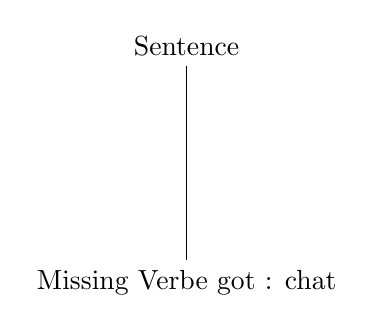
\begin{tikzpicture}
\node{Sentence}[sibling distance = 3cm, level distance = 3cm, align=center]
child {node {Missing Verbe got : chat}};
\end{tikzpicture}
\end{center}
\begin{center}
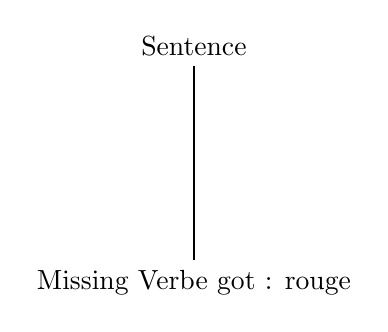
\begin{tikzpicture}
\node{Sentence}[sibling distance = 3cm, level distance = 3cm, align=center]
child {node {Missing Verbe got : rouge}};
\end{tikzpicture}
\end{center}
\begin{center}
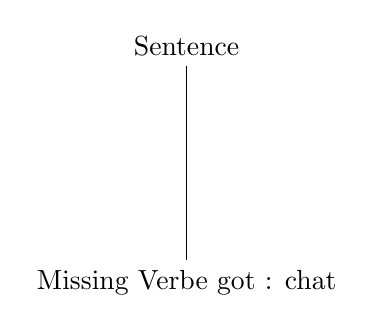
\begin{tikzpicture}
\node{Sentence}[sibling distance = 3cm, level distance = 3cm, align=center]
child {node {Missing Verbe got : chat}};
\end{tikzpicture}
\end{center}
\begin{center}
\begin{tikzpicture}
\node{Sentence}[sibling distance = 3cm, level distance = 3cm, align=center]
child { node {GV \\ O3, m, s} child { node {Sujet \\ m, s} child { node {GN \\ m, s} child { node {Determinant \\ m, s} child {node {le}}}child { node {Adjectif \\ m, s} child {node {petit}}}child { node {Nom \\ m, s} child {node {chat}}}child { node {Adjectif \\ e, s} child {node {rouge}}}}}child { node {Verbe \\ i, \_, \_, \_, \_, \_, a, Ip, 3s} child {node {dort}}}};
\end{tikzpicture}
\end{center}
\end{document}
